\begin{figure*}[thp]
	\center
	\begin{subfigure}{0.75\textwidth}
		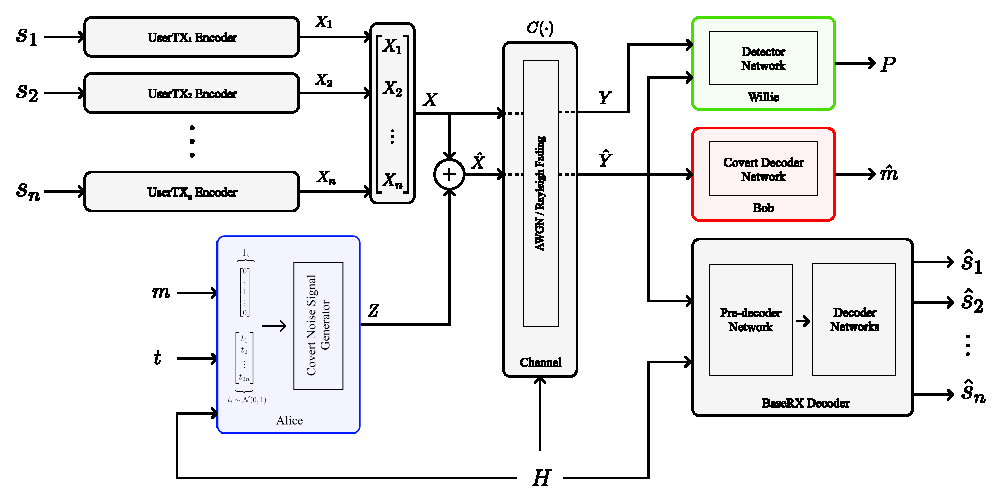
\includegraphics[width=\linewidth]{figs/multi_system_architecture}
	\end{subfigure}
	\\
	\caption{Overall architecture of our system model in the multi-user scenario. Alice is communicating with Bob by generating covert noise signals without disturbing the communication between other \(n\)-UserTXs and BaseRX; meanwhile, Willie tries to distinguish covert and normal signals (Colored components are under the control of covert users and gray components are the non-modifiable parts of the system).}	
	\label{fig:multi_system_architecture}
\end{figure*}


\section{Multi-User System Model}
\label{s:multi-model}
Now that we discussed the single-user system model and evaluation results, in this section, we are going to talk about the second part of our article that covers a multi-user communication model scenario. Many parts of this model will be similar to what we described in (=\ref{s:single-model}) except that with more than one user sharing the channel, both normal and covert users now have to account for signal interference to communicate reliably. This will result in a much more complex optimization problem when we are training normal and covert users' neural networks.

In figure \ref{fig:multi_system_architecture} you can see the overall architecture of our multi-user communication system. The system compromises multiple separate normal transmitters (UserTXs) that are sending signals to a central base station receiver (BaseRX). Each UserTX and BaseRX together form an autoencoder model wherein UserTX is the encoder and BaseRX acts as the decoder network. The objective of our work, again, is to establish a covert channel between two covert users, namely Alice and Bob, on top of this normal communication channel without leaving any impact on any of these normal communicating parties. Normal transmitters each use their own encoder network to encode a binary message to a vector of signals. Their networks share no parameters and the message they are sending is unknown to the other transmitters of the system. At the time of transmission, they all send their signals simultaneously and since they are sharing the same channel, there will be channel interference. As for the channel effect, the two channel models of AWGN and Rayleigh fading are considered. When signals pass through the channel, they get distorted both by the channel effects and the channel interference. These noisy signals are then received at BaseRX, all at the same time. BaseRX uses its decoder network to reconstruct the messages sent by the transmitters from the received signals. Alice and Bob's objective is no different from what we mentioned previously in our single-user system model. Their goal is to construct a hidden communication channel and embody their messages inside normal signal transmissions of the communication system in form of an added noise. In order to remain covert, they have to ensure that these added perturbations make no disturbance to the ongoing normal communication (i.e. increasing the error rate of communication) and leave no statistical traces behind from an observer's perspective. Thus, there is an observer (Willie) whose objective is to continuously look into the transmitted signals over the channel and raise an alarm whenever covert communication is deemed to be present. We represent all these roles by DNNs that are collaboratively trained to establish a covert communication channel. By using a generative model, Alice embeds its confidential message into a covert noise vector which will be added to the signals being transmitted over the channel. Bob receives this signal and uses its decoder network to extract the covert message. Unlike our single-user system model wherein covert users were devised independently of what the channel model is, here they use different neural networks depending on the channel model. Channel statistics are monitored by the observer of the system (Willie). Willie's objective is to detect any anomaly that in this case would be a covert communication taking place. Thus, if Alice and Bob construct their covert signals in such a way that Willie fails to tell them apart from the normal signals, then the covertness of their communication is safeguarded.

\textbf{Background on Multi-User Autoencoder Systems}: A multi-user autoencoder communication system is just an extended version of a single-user system with either multiple transmitters and receivers or multiple transmitters and a central receiver. We considered the latter in our work. Similar to the single-user system, in this model each of these encoders (transmitters) first maps \(k\) bits of data into a message \(s_i\) where \(s \in \{1,...,M\}\), \(M = 2^k\), and \(i\) is the index of the transmitter. Then each transmitter takes this transformed message as an input and generates a signal \(x_i = E_i(s_i) \in \mathbb{R}^{2n}\), which is a real-valued vector. This \(2 \times n\)-dimensional real-valued vector can be treated as an \(n\)-dimensional complex vector where \(n\) is the number of channel uses that are needed for the signal to be transmitted over. Next, there will be distortions caused by the channel interference and effects. For the AWGN channel, transmitted signals are added together and the channel's noise effect \(z\) gets added to this mixed signal vector. Thus, each transmitter's received signal at the receiver, carrying the noise of the channel and interference, can be expressed as \(y_i = \sum_{i=0}^{m}x_i + z_i\) where \(n_{tx}\) is the number of transmitters. In Rayleigh fading channel case, signals are simultaneously faded and mixed by being multiplied by the channel matrix and the resulting vector of signals for each transmitter can be expressed as \(y_i = h_i \cdot x + z_i\), where \(h_i\) is channel coefficients for the \(i^{th}\) transmitter's signals (\(h\) itself is a vector of size \(n_{tx}\) wherein each element \(h_{i_j}\sim \mathcal{CN}(0, 1)\)) and \(x\) is a vector containing all transmitters' encoded signals. Transmitted signals that have gone through the channel are received at the decoder (receiver) and then get passed to a transformation function \(D: \mathbb{R}^{2n} \rightarrow M \) along with the channel matrix \(h\) and eventually, the reconstructed version of the message \(s\), which is denoted as \(\hat{s} = D(y, h)\), is obtained.

\begin{figure*}[!tp]
	\center
	\begin{subfigure}{0.45\textwidth}
		\includegraphics[width=\linewidth]{figs/multi_autoencoder_bler_awgn}
		\caption{AWGN channel}
	\end{subfigure}
	\begin{subfigure}{0.45\textwidth}
		\includegraphics[width=\linewidth]{figs/multi_autoencoder_bler_rayleigh}
		\caption{Rayleigh fading channel}	
	\end{subfigure}
	\caption{Trained Autoencoders' BLERs for different numbers of users over a range of SNR values in our multi-user system.}
	\label{fig:multi_autoencoder_bler}
\end{figure*}


\section{Covert Model for Multi-User Systems}
The covert communication starts with Alice sending a binary secret message \(m\) to Bob. This message is first encoded to a one-hot vector and then passed to a generator network to produce a covert signal noise signal \(\hat{z}\). This then will be added to a vector of normal signals \(x\), which contains signals from all the transmitters before transmission. Hence, the resulting covert signal can be denoted as:
\begin{equation}
	\hat{x}_i = x_i + \hat{z}.
\end{equation}

Afterwards, this signal is transmitted over the channel. We have considered two channel models of AWGN and Rayleigh for this model. Each of these channel models has an effect on the signal that we denote as a mapping function \(C(\cdot)\).

\textit{AWGN Channel Output}: In this channel mode, the channel effect is applied by adding a noise vector \(z \sim \mathcal{N}(0, \sigma_{chl}^2)\) to the signal. Therefore, the channel function \(C(\cdot)\) and the channel output \(\hat{y}\) can be represented as:
\begin{equation}
	\hat{y}_i = C(\hat{x}_i) = \sum_{i=0}^{m}\hat{x}_i + z_i.
\end{equation}

\textit{Rayleigh Channel Output}: For the Rayleigh fading channel model, a flat block fading channel is considered wherein each code-word \(\hat{x}_i\) is assumed to be faded independently by fading coefficient \(h_{i_j}\). Consequently, the channel function \(C(\cdot)\) and the final covert signal \(\hat{y}\) is written as:
\begin{equation}
	\hat{y}_i = C(\hat{x}_i) = h_i \cdot \hat{x} + z_i.
\end{equation}

After the signal goes through the channel, Bob receives it at its receiver. With the help of his decoder network, he extracts the covert message \(\hat{m}\) from the covert signal \(\hat{y}\). Similarly, BaseRX receives the same signal and passes it to its decoder to reconstruct the message \(\hat{s}\).

Willie as an observer of the system continuously monitors the channel. His job is to label the received signals as covert and normal. By gradually altering the covert signals and tracking how Willie's confidence in detecting covert signals changes, Alice will steadily learn to better cover up its covert signals. Technically, Alice tries to make covert signals statistically similar to normal signals so that they become indistinguishable.

\subsection{General Formulation}

To have reliable working covert communication between Alice and Bob, Bob needs to learn how to decode the messages that Alice transmits. In this regard, the first objective of Bob is to minimize the reconstruction error of the covert message \(m\) sent by Alice. Similar to what we proposed in our single-model system, Alice maps binary covert messages \(m\) to a vector of covert signals \(\hat{z}\) using a generative model. The only difference in Alice's network from before is that now Alice needs the channel matrix \(h\) when she is operating over Rayleigh fading channel. Therefore, given \(A(\cdot)\) as Alice's generative model, the produced covert signal for AWGN and Rayleigh channels are \(\hat{z}_{m, t} = A(m, t)\), \(\hat{z}_{m, t, h} = A(m, t, h)\), respectively. Now let \(B(\cdot)\) be the function of Bob's decoder network, then below loss function ensures the above objective:
\begin{equation}
	\begin{aligned} \label{multi_bob_loss}
		\mathcal{L}_{Bob} & = \mathbb{E}_{m}[H(\hat{m}, m)] \\
		& = \mathbb{E}_{m}[H(B(\hat{y}), m)] \\ 
		& = \mathbb{E}_{m}[H(B(C(\hat{x}), m)] \\ 
		& = \begin{cases} 
			\mathbb{E}_{m}[H(B(C(A(m, t) + x)), m)] & AWGN \\
			\mathbb{E}_{m}[H(B(C(A(m, t, h) + x)), m)] & Rayleigh.
			\end{cases}
	\end{aligned}
\end{equation}

We use this equation to train both Alice's and Bob's networks by freezing one or the other's network parameters. From an observer's point of view, any abnormal increase in communication's error rate would indicate an anomaly in the system and in our case a covert communication. Therefore, Alice needs to tune its covert signals so that its impact on other normal transmitters communication is minimum. This we will achieve by using the below loss function for Alice's network:
\begin{equation}
	\begin{aligned} \label{multi_alice_user_loss}
		\mathcal{L}_{BaseRX} & = \sum_{i=0}^{i=m}\mathbb{E}_{m}[H(\hat{s}_i, s_i)] \\
		& = \sum_{i=0}^{i=m}\mathbb{E}_{m}[H(D(\hat{y}_i), s_i)] \\
		& = \sum_{i=0}^{i=m}\mathbb{E}_{m}[H(D(C(\hat{z}_i + x_i)), s_i)] \\
		= \sum_{i=0}^{i=m} & \begin{cases} 
			\mathbb{E}_{m}[H(D(C(A(m, t) +  x_i)), s_i)] & AWGN \\
			\mathbb{E}_{m}[H(D(C(A(m, t, h) + x_i), h), s_i)] & Rayleigh. \\
		\end{cases} 
	\end{aligned}
\end{equation}
 
With the two equations above, the reliability of covert communication will be achieved and we will have covertness to some extent. Yet, we need to account for an observer (Willie) who will be appointed to observe the communication channel closely to detect if any probable covert or abnormal communication is taking place. Thus, there is a third loss function for Willie denoted as:
\begin{equation}
	\begin{aligned} \label{multi_willie_loss}
		\mathcal{L}_{Willie} & = \mathbb{E}_{m}[H(\hat{y}, y)] \\
		& = \mathbb{E}_{m}[H(C(\hat{x}), C(x))] \\
		& = \begin{cases}
			\mathbb{E}_{m}[H(C(A(m,t) + x), C(x))] & AWGN \\
			\mathbb{E}_{m}[H(C(A(m,t,h) + x), C(x))] & Rayleigh.
			\end{cases}
	\end{aligned}
\end{equation}

Using this loss function, Willie will have enough data to learn how to differentiate covert and normal signals. Since it is vital for covert users to keep their transmissions hidden from the observer of the system, they can exploit the same loss function declared above to increase the covertness of their communication. By putting these constraints all together and using equation (\ref{alice_loss}), we now have the final optimization formula for training Alice's network.

\subsection{Neural Network Architecture}
There is not much difference in our models' architectures from what we proposed in the single-user model except for the decoder part of the autoencoder's network and a few extra parameters for Alice's network. We will explain each model's structure in detail in the following subsections.

\textbf{Autoencoders' Networks}: The input to each autoencoder model is a different binary message \(s\) of size \(k\) bits and the output is a reconstructed version of that message \(\hat{s}\). Figure \ref{fig:mutli_autoencoder_architecture} depicts the overall architecture of our multi-user autoencoder model. First, each autoencoder model transforms the given message into its one-hot representation and then encodes it to a vector of signals of size \(2 \times n\), where \(n\) is the number of channel uses for the whole system. Signals are then distorted using a mapping function that corresponds to the channel model effects. On the receiver side, there is a central decoder that receives all transmitter's signals at once and extracts the message of each by passing the signals through its neural network. When the channel model is Rayleigh fading, the decoder equalizes the signals using zero-forcing technique with the channel matrix before passing the signals to its network. Note that there are plenty of more complex equalization functions that can be used, however, optimizing the performance of the autoencoder model is not the focus of this article.

\textbf{Alice's Network}: Alice takes a random trigger \(t\), and a covert message \(m\), which is one-hot encoded, and then uses her generator model to produce a covert noise signal \(\hat{z}\). In the case of the Rayleigh fading channel, the channel matrix is also fed to her network. Next, she adds this to normal signals \(x_i\)s that are carrying the normal messages between normal users of the system. Alice's generator model consists of dense layers with ReLU and Tanh activation functions. The first layer of her model takes a trigger input \(t\), a covert message \(m\). Channel matrix \(h\) is also an input to her network when the channel is Rayleigh fading. Followed are multiple fully connected layers that are to extract the useful features and do the encoding process. The last layer of the network does a dimension transformation so that the generated covert signal \(\hat{z}\) complies with the dimension of normal signals \(x_i\)s on the channel. 

\textbf{Bob's Network}: A noisy version of covert signal \(\hat{y}\) is received at Bob's decoder network. His objective is to extract the secret message by doing classification on the signal. This received signal first goes through the first layer of his network, which is a wide dense layer with a Tanh activation function, and its aim is to increase the input's feature space. Then the data is passed through multiple 1-Dimensional Convolutional (1D Conv) layers that allow Alice and Bob to develop a mutually learned coding. The last two dense layers of Bob's network are for domain remapping from the learned feature space to the covert message domain space. After a successful training, Bob will eventually learn to decode the messages from covert signals by doing classification.


\textbf{Willie's Network}: Whatever signal Bob receives, Willie receives as well. He also has access to the normal signals \(y\) and by doing binary classification on these signals and the covert signals \(\hat{y}\), he outputs a probability vector \(P\) that shows how probable it is for the signals to be normal or covert. Willie's network architecture is chosen to be the same as the Bob's except for the last layer, which has a Sigmoid activation function instead of a Softmax. By having equally sized networks, we can ensure that Bob and Willie will have the same capacity for learning, and thus can compete in a fair way.

\begin{figure}[tp!]
	\center
	\begin{subfigure}{0.5\textwidth}
		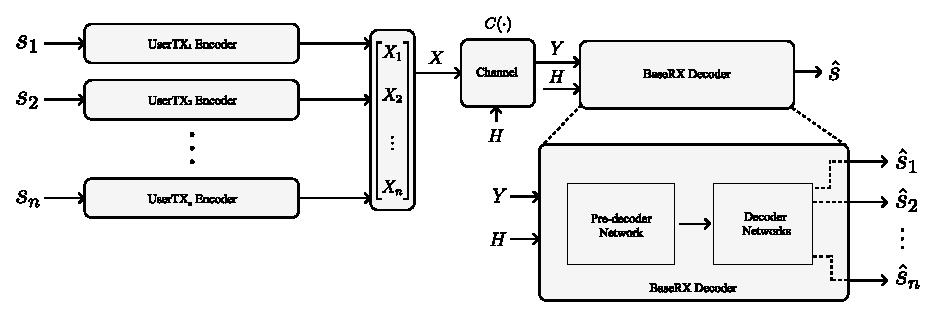
\includegraphics[width=.98\linewidth]{figs/multi_autoencoder_architecture}
	\end{subfigure}
	\\
	\caption{Detailed architecture of BaseRX's decoder network. Signals from all receivers are passed through the pre-decoder network and then each transmitter's message is extracted separately using the decoder networks.}	
	\label{fig:multi_autoencoder_architecture}
\end{figure}